% Created 2024-03-25 Mon 00:30
% Intended LaTeX compiler: pdflatex
\documentclass[a4paper,11pt]{exam}
\usepackage[utf8]{inputenc}
\usepackage[T1]{fontenc}
\usepackage{graphicx}
\usepackage{longtable}
\usepackage{wrapfig}
\usepackage{rotating}
\usepackage[normalem]{ulem}
\usepackage{amsmath}
\usepackage{amssymb}
\usepackage{capt-of}
\usepackage{hyperref}
\usepackage[T1]{fontenc}
\usepackage{titling}
\usepackage{url}
\usepackage{amsmath,amsthm,amssymb}
\usepackage{titling}
\usepackage{url}
\usepackage{amsmath,amsthm,amssymb}
\usepackage{graphicx}
\usepackage{graphics}
\usepackage{listings}
\usepackage[dvipsnames]{xcolor}
\usepackage{tabularx}
\usepackage{ragged2e}
\usepackage{courier}
\usepackage{textcomp}
\usepackage{circuitikz}
\usepackage{tikz}
\usepackage{enumitem}
\usepackage{karnaugh-map}
\usepackage{bytefield}
\usepackage{mathrsfs}
\usepackage{cancel}
\usepackage[linesnumbered,ruled,vlined]{algorithm2e}
\usepackage{hyperref}
\usepackage{environ}
\usepackage{listings}
\usepackage{algorithm}
\usepackage{algpseudocode}
\lstset{breaklines=true, basicstyle=\ttfamily\tiny, frame=single, escapeinside={(*@}{@*)}}
\usepackage[margin=0.75in]{geometry}
\author{Miguel Gomez U1318856}
\date{2024-03-25 00:30:34}
\title{Homework Assignment \# 3}
\hypersetup{
 pdfauthor={Miguel Gomez U1318856},
 pdftitle={Homework Assignment \# 3},
 pdfkeywords={},
 pdfsubject={},
 pdfcreator={Emacs 28.2 (Org mode 9.4.6)}, 
 pdflang={English}}
\begin{document}

\maketitle
\tableofcontents

\newpage

\section{HW3 - Problem 1}
\label{sec:org8e7941e}
design an elliptic curve crypto-cipher over a Galois field of the type \(\mathbb{F}_{2^k}\).  Implement the key generation, encryption and decryption modules in Singular, and demonstrate the correct simulation.
\subsection{a) what are \(\alpha^4 , \alpha^5 , \alpha^6\) when reduced (mod \(P(\alpha)\))}
\label{sec:org6c04178}
Consider the finite field \(\mathbb{F}_{2^k} \equiv \mathbb{F}_{2}[x]\) (mod \(P(x)\)) where \(P(x) = x^3 + x^2 + 1\). Let \(\alpha\) be a root of \(P(x)\), i.e. \(P(\alpha) = 0\). Note that \(P(x)\) is indeed a primitive polynomial. Using Singular, enumerate the field elements \(F_8 = {0, \alpha^7 = 1, \alpha, \alpha^2, \alpha^3 = \alpha^2 + 1, \alpha^4 =?, . . . , \alpha^6 =?}\). In other words, what are \(\alpha^4 , \alpha^5 , \alpha^6\) when reduced (mod \(P(\alpha)\))?

\begin{verbatim}
start=$(date +%s.%N)
Singular ./sing/point_enumeration.sing | grep -v -e "\*\* loaded\|\*\* library"
end=$(date +%s.%N)
echo "Execution Time: $(echo "$end - $start" | bc) seconds"
\end{verbatim}

As can be seen in the output below, \(\alpha^4,\ \alpha^5,\ \alpha^6\) are as follows:

\begin{align*}
\alpha^4 &= \alpha^2+\alpha+1\\
\alpha^5 &= \alpha+1\\
\alpha^6 &= \alpha^2+\alpha
\end{align*}


\[
\subsubsection{output of point-enumeration.sing results}
\begin{lstlisting}[language=Singular]
                     SINGULAR                                 /  Development
 A Computer Algebra System for Polynomial Computations       /   version 4.3.2
                                                           0<
 by: W. Decker, G.-M. Greuel, G. Pfister, H. Schoenemann     \   Feb 2023
FB Mathematik der Universitaet, D-67653 Kaiserslautern        \
// ** executing /home/speedy/repos/singular/git/Singular/Singular/Singular/.libs/../LIB/.singularrc
// ** but for functionality you may wish to change to the new
// ** format. Please refer to the manual for further information.
================================
when x = 0
poly f is:
y2+1
poly f factorizes as follows:
[1]:
   _[1]=1
   _[2]=y+1
[2]:
   1,2
================================
when x = A^0, : x = 1
P1(x,y) = (1,y2+(A2))
================================
when x = A^1, : x = (A)
P1(x,y) = ((A),1)
P2(x,y) = ((A),y+(A+1))
================================
when x = A^2, : x = (A2)
P1(x,y) = ((A2),(A))
P2(x,y) = ((A2),y+(A2+A))
================================
when x = A^3, : x = (A2+1)
P1(x,y) = ((A2+1),(A+1))
P2(x,y) = ((A2+1),y+(A2+A))
================================
when x = A^4, : x = (A2+A+1)
P1(x,y) = ((A2+A+1),(A))
P2(x,y) = ((A2+A+1),y+(A2+1))
================================
when x = A^5, : x = (A+1)
P1(x,y) = ((A+1),0)
P2(x,y) = ((A+1),y+(A+1))
================================
when x = A^6, : x = (A2+A)
P1(x,y) = ((A2+A),1)
P2(x,y) = ((A2+A),y+(A2+A+1))
================================
when x = A^7, : x = 1
P1(x,y) = (1,y2+(A2))
================================
Auf Wiedersehen.
Execution Time: .060719112 seconds
\end{lstlisting}
\]




\subsection{b)  Enumerate all the points on the curve}
\label{sec:org7110c0f}

\begin{verbatim}
start=$(date +%s.%N)
Singular ./sing/point_gen.sing | grep -v -e "\*\* loaded\|\*\* library"
end=$(date +%s.%N)
echo "Execution Time: $(echo "$end - $start" | bc) seconds"
\end{verbatim}


\[
\subsubsection{output of point\_gen.sing results}
\begin{lstlisting}[language=Singular]
                     SINGULAR                                 /  Development
 A Computer Algebra System for Polynomial Computations       /   version 4.3.2
                                                           0<
 by: W. Decker, G.-M. Greuel, G. Pfister, H. Schoenemann     \   Feb 2023
FB Mathematik der Universitaet, D-67653 Kaiserslautern        \
// ** executing /home/speedy/repos/singular/git/Singular/Singular/Singular/.libs/../LIB/.singularrc
// ** but for functionality you may wish to change to the new
// ** format. Please refer to the manual for further information.
P = ((A2+1), (A+1))
Calling doubleP on P
received/ 2P:
2P = ((A2), (A2+A))
3P = ((A2+A), (A2+A+1))
4P = ((A), (A+1))
5P = ((A+1), 0)
6P = ((A2+A+1), (A2+1))
7P = (0, 1)
8P = ((A2+A+1), (A))
9P = ((A+1), (A+1))
10P = ((A), 1)
11P = ((A2+A), 1)
12P = ((A2), (A))
13P = ((A2+1), (A2+A))
14P = (0, 0)
15P = ((A), (A2+A+1))
16P = ((A2+1), (A2+A))
Auf Wiedersehen.
Execution Time: .074262521 seconds
\end{lstlisting}
\]


Shown above is the enumeration of the points and below they are added with nicer formatting.

\begin{align*}
  P &= (\alpha^2+1, \alpha+1)\\
  2P &= (\alpha^2, \alpha^2+\alpha)\\
  3P &= (\alpha^2+\alpha, \alpha^2+\alpha+1)\\
  4P &= (\alpha, \alpha+1)\\
  5P &= (\alpha+1, 0)\\
  6P &= (\alpha^2+\alpha+1, \alpha^2+1)\\
  7P &= (0, 1)\\
  8P &= (\alpha^2+\alpha+1, \alpha)\\
  9P &= (\alpha+1, \alpha+1)\\
  10P &= (\alpha, 1)\\
  11P &= (\alpha^2+\alpha, 1)\\
  12P &= (\alpha^2, \alpha)\\
  13P &= (\alpha^2+1, \alpha^2+\alpha)\\
  14P &= (0, 0)
 \end{align*}

\subsection{c)  Identify a point \(P(x, y)\) that acts as a primitive element}
\label{sec:org7dfe4e5}

This result above provided by the Singular procedure proves that we can generate the points on the curve as well as proving that our starting point below is a generator.

\begin{align*}
P &= (\alpha^3,\alpha^5) = (\alpha^2 + 1, \alpha + 1)
\end{align*}


\subsection{d) Is its inverse point \(P^{-1}\) also a generator of G?}
\label{sec:org6d7057b}
Let a point \(P(x1 , y1)\) be a generator of \(G = \left<E, +\right>\). Is its inverse point \(P^{-1}\) also a generator of \(G\)? If yes, then prove it. Otherwise, give a counterexample.


\begin{verbatim}
start=$(date +%s.%N)
Singular ./sing/point_inversion.sing | grep -v -e "\*\* loaded\|\*\* library"
end=$(date +%s.%N)
echo "Execution Time: $(echo "$end - $start" | bc) seconds"
\end{verbatim}


\[
\subsubsection{output of inversion results}
\begin{lstlisting}[language=Singular]
                     SINGULAR                                 /  Development
 A Computer Algebra System for Polynomial Computations       /   version 4.3.2
                                                           0<
 by: W. Decker, G.-M. Greuel, G. Pfister, H. Schoenemann     \   Feb 2023
FB Mathematik der Universitaet, D-67653 Kaiserslautern        \
// ** executing /home/speedy/repos/singular/git/Singular/Singular/Singular/.libs/../LIB/.singularrc
// ** but for functionality you may wish to change to the new
// ** format. Please refer to the manual for further information.
printing 1P:
((A2+1), (A+1))
printing 2P:
((A2), (A2+A))
printing 3P:
((A2+A), (A2+A+1))
printing 4P:
((A), (A+1))
printing 5P:
((A+1), 0)
printing 6P:
((A2+A+1), (A2+1))
printing 7P:
(0, 1)
printing 8P:
((A2+A+1), (A))
printing 9P:
((A+1), (A+1))
printing 10P:
((A), 1)
printing 11P:
((A2+A), 1)
printing 12P:
((A2), (A))
printing 13P:
((A2+1), (A2+A))
printing 14P:
(0, 0)
Auf Wiedersehen.
Execution Time: .041399348 seconds
\end{lstlisting}
\]







\subsection{e) simulate El Gamal encipherment}
\label{sec:org8895308}
Using the solutions to the above questions, you will now simulate El Gamal encipherment over the above elliptic curve.

\subsubsection{selecting parameters for encryption}
\label{sec:orgec72a22}
Based on Fig.1, which is reproduced from our slides, select \(e_1\) as a generator of \(G = \left<E, +\right>\). Select integers \(d\), \(r\), such that \(d \ne r\).

\begin{center}
\begin{figure}[h]
    \centering
    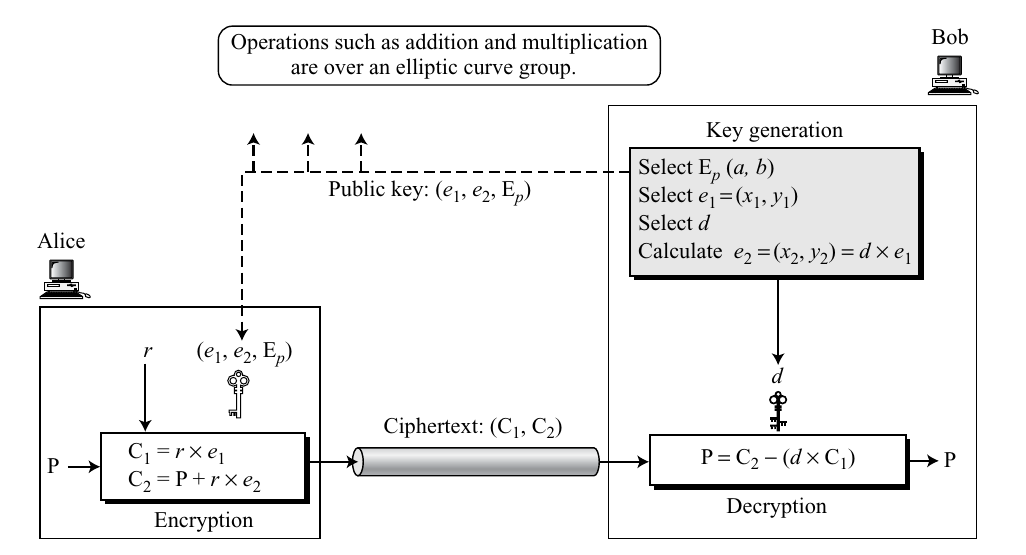
\includegraphics[width=16cm]{./images/fig1_hw3.png}
    \caption{El Gamal over ECC}
    \label{fig:fig1_hw3}
  \end{figure}
\end{center}

\subsubsection{Selecting plain-text}
\label{sec:org14954c4}
Select the plaintext \(P\) as a point on the elliptic curve. Compute \(C_1\) , \(C_2\) to demonstrate encryption. [Avoid \(P = (0, 1)\), as it is a trivial point on our non-supersingular curves over \(\mathbb{F}_{2^k}\) ].

\subsubsection{Demonstrate decryption by re-obtaining the plaintext \(P\)}
\label{sec:org650e759}

\subsection{f) Notes:}
\label{sec:orgab27071}
Note: Implement the above in Singular. Please make use of “procedures” in Singular to make your code Modular. Print out the relevant parts of your computation to make it easier for me and  the grader  to grade it when I run your code.  Attach a README to help me understand how to run your code.  Also,  in a PDF file, please  describe  (briefly)  which points you are using as generators, what are your keys \(e_1\) , \(e_2\) , \(d\), \(r\) and the corresponding \(P\), \(C_1\), \(C_2\) values. 

\subsection{g) Permissions for using skeleton provided}
\label{sec:org8cdbd85}
It goes without saying: feel free to borrow inspirations from the Singular files I used to give you a demo of ECC El Gamal in class; those Singular files are uploaded on Canvas: ecc-f8-example.sing.


\section{Problem 2}
\label{sec:orge58b6d4}
In this question, you will design a digital logic circuit that performs point doubling \(R = 2P\)  (not point addition!) over elliptic curves using the projective coordinate system. You will first design (or re-use from HW 2) a multiplier circuit, use it as a building block to perform doubling. You will implement your design in Verilog or VHDL, and demonstrate that point addition is being performed correctly.

\subsection{a) Defining field and terms}
\label{sec:org23554a5}
We will use the same finite field as in the previous question: F8 ≡ F2 [x] (mod P(x) =x3 + x2 + 1) with P(α) = 0. Denote the degree of P(x) as k; of course, here k = 3.

\subsection{b) Design multiplier}
\label{sec:org5bea844}
Design a k = 3 bit finite field multiplier that takes A = \{a2, a1 , a0 \} and B = \{b2 , b1 , b0 \} as 3-bit inputs, and produces Z = \{z2 , z1 , z0\} as a 3-bit output. Note that we will have:

\begin{align*}
A &= a_0 + a_1 \alpha + a_2\alpha^2\\
B &= b_0 + b_1 \alpha + b_2\alpha^2\\
Z &= z_0 + z_1 \alpha + z_2\alpha^2
\end{align*}

Such that \(Z = A \cdot B\) mod \(P(\alpha))\). Of course, you have already designed 2 multipliers in the last HW (Mastrovito and Montgomery). Just pick whichever one you like. Also, please double check that the primitive polynomial that you used in the design of HW 2 was indeed \(P(x) = x^3 + x^2 + 1\).


\subsection{c) Implementation in Verilog}
\label{sec:orgbd97ada}
Implement the design in Verilog/VHDL (GFMult(A, B, Z) module) and demonstrate/simulate using a testbench the following input-output combinations:


\begin{align*}
 A &= (0, 1, 0) = \alpha \\
 B &= (1, 0, 0) = \alpha^2\\
 Z &= (1, 0, 1) = \alpha^2 + 1
\end{align*}
\subsubsection{2.}
\label{sec:orgc8a414c}

\begin{align*}
A &= \alpha^2 + 1\\
B &= \alpha^2 + \alpha + 1
\\Z &= ?
\end{align*}
\subsection{d) Design Squarer}
\label{sec:org6ceee77}
Using your GFMult module, create a squarer module by connecting \(A = B\) inputs; call it the
GFSQR module.

\subsection{e) Design GFADD}
\label{sec:orgaa33f24}
Design a GFADD(A, B, Z) Verilog Module, such that \(Z = A+B\) over \(\mathbb{F}_8\) . [Remember, addition
in Galois Fields is just a bit-wise XOR].

\subsection{f) Implement Point doubling in projective coordinates}
\label{sec:orgd0213ee}
In the lecture slides (ECC-GF.pdf), I have given you the correct formulas for point addition
and doubling operations. Implement a Verilog Module to perform point doubling over projective
coordinates. Your PointDouble\((X_3,Y_3,Z_3,X_1,Y_1,Z_1)\) Verilog/VHDL module should instan-
tiate GFADD, GFMult, GFSQR modules accordingly to compute each of the 3-bit \(X_3, Y_3, Z_3\)
outputs.

\subsection{g) DFG}
\label{sec:orgfeb249a}
Draw a Data Flow Graph (DFG) for \(X_3, Y_3, Z_3\), using the 3 operators, to show how your
adders, multipliers and squarers are organized.

\subsection{h) Simulation and example demonstrations}
\label{sec:orge2dfc6f}
 Demonstrate that your PointDouble() module correctly computes the doubling of the
following affine points:

\subsubsection{Defining projective plane}
\label{sec:orgb8fd7ec}
Pick \(Z_1 = 1\) to keep computations simple. Note that since each coordinate of a point is
in \(\mathbb{F}_8\) , each of \(X_1, Y_1, Z_1\) is a 3-bit vector.

\subsubsection{\(P = (\alpha, 1)\) simulate \(2P\)}
\label{sec:orgc66fb16}
For affine point \(P = (\alpha, 1)\), simulate \(2P\) on your Verilog Testbench. What is \(2P\)?
\subsubsection{\(P = (\alpha^3, \alpha + 1)\) simulate \(2P\)}
\label{sec:orgd6c437e}
For affine point \(P = (\alpha^3, \alpha + 1)\), simulate \(2P\) on your Verilog Testbench. What is \(2P\) for
this case?
\subsubsection{Notes:}
\label{sec:org024a86e}
Note that \((X_1 , Y_1 , Z_1 )\) computed by your circuit is actually \((\frac{X_1}{Z_1}, \frac{Y_1}{Z_1})\) in the affine
space! You can of course check your answer with Singular.
\end{document}